\documentclass[11pt, a4paper,]{report}
\usepackage[italian]{babel}
\usepackage{lipsum}
\usepackage{multicol}
\usepackage{amsthm}
\usepackage{listings}
\usepackage{float}
\usepackage{amssymb}
\usepackage{dirtree}
\theoremstyle{definition}
\newtheorem{definition}{Definizione}[section]
\usepackage{graphicx}
\usepackage{wrapfig}
\usepackage{xcolor}
\usepackage[citestyle=numeric]{biblatex}
\addbibresource{database.bib}
\usepackage[utf8]{inputenc}
\usepackage[hidelinks, colorlinks]{hyperref}
\usepackage{changepage}
\usepackage{longtable}
\usepackage{pdfpages}
\usepackage{layout}
\usepackage{geometry}
\geometry{a4paper,left=3cm, right=3cm, top=3cm,bottom=3cm, headheight=0cm}
\graphicspath{{images/}}
\hypersetup{allcolors=black}
\begin{document}
	\definecolor{color_29791}{rgb}{0,0,0}
	\begin{picture}(0,0)(0,0)
		\put(252.5999,-116.88){
\includegraphics[width=60pt,height=56.99998pt]{latexImage_7a11001d2473257fa9c3a53b3d87b883.png}}
		\put(312.6,-116.88){\fontsize{12}{1}\usefont{T1}{cmr}{m}{n}\selectfont\color{color_29791} }
		\put(282.6,-128.16){\fontsize{12}{1}\usefont{T1}{cmr}{m}{n}\selectfont\color{color_29791} }
		\put(282.6,-141.96){\fontsize{12}{1}\usefont{T1}{cmr}{m}{n}\selectfont\color{color_29791} }
		\put(282.6,-155.76){\fontsize{12}{1}\usefont{T1}{cmr}{m}{n}\selectfont\color{color_29791} }
		\put(282.6,-169.56){\fontsize{12}{1}\usefont{T1}{cmr}{m}{n}\selectfont\color{color_29791} }
		\put(117.36,-185.28){\fontsize{14.04}{1}\usefont{T1}{cmr}{m}{n}\selectfont\color{color_29791}UNIVERSITÀ DEGLI STUDI GUGLIELMO MARCONI }
		\put(41.64,-199.44){\fontsize{12}{1}\usefont{T1}{cmr}{m}{n}\selectfont\color{color_29791} }
		\put(243.12,-213.24){\fontsize{12}{1}\usefont{T1}{cmr}{m}{n}\selectfont\color{color_29791}FACOLTA’ DI  }
		\put(218.04,-227.04){\fontsize{12}{1}\usefont{T1}{cmr}{m}{n}\selectfont\color{color_29791}CORSO DI LAUREA IN  }
		\put(41.64,-240.84){\fontsize{12}{1}\usefont{T1}{cmr}{m}{n}\selectfont\color{color_29791} }
		\put(41.64,-254.64){\fontsize{12}{1}\usefont{T1}{cmr}{m}{n}\selectfont\color{color_29791} }
		\put(41.64,-268.4399){\fontsize{12}{1}\usefont{T1}{cmr}{m}{n}\selectfont\color{color_29791} }
		\put(41.64,-282.2399){\fontsize{12}{1}\usefont{T1}{cmr}{m}{n}\selectfont\color{color_29791} }
		\put(41.64,-296.0399){\fontsize{12}{1}\usefont{T1}{cmr}{m}{n}\selectfont\color{color_29791} }
		\put(41.64,-309.8399){\fontsize{12}{1}\usefont{T1}{cmr}{m}{n}\selectfont\color{color_29791} }
		\put(41.64,-323.6399){\fontsize{12}{1}\usefont{T1}{cmr}{m}{n}\selectfont\color{color_29791} }
		\put(282.6,-337.4399){\fontsize{12}{1}\usefont{T1}{cmr}{m}{n}\selectfont\color{color_29791} }
		\put(41.63998,-351.2399){\fontsize{12}{1}\usefont{T1}{cmr}{m}{n}\selectfont\color{color_29791} }
		\put(282.6,-365.0399){\fontsize{12}{1}\usefont{T1}{cmr}{m}{n}\selectfont\color{color_29791} }
		\put(282.6,-378.8398){\fontsize{12}{1}\usefont{T1}{cmr}{m}{n}\selectfont\color{color_29791} }
		\put(282.6,-392.6398){\fontsize{12}{1}\usefont{T1}{cmr}{m}{n}\selectfont\color{color_29791} }
		\put(41.63998,-406.4398){\fontsize{12}{1}\usefont{T1}{cmr}{m}{n}\selectfont\color{color_29791} }
		\put(282.6,-420.2398){\fontsize{12}{1}\usefont{T1}{cmr}{m}{n}\selectfont\color{color_29791} }
		\put(282.6,-434.0398){\fontsize{12}{1}\usefont{T1}{cmr}{m}{n}\selectfont\color{color_29791} }
		\put(200,-401.56){\fontsize{15.96}{1}\usefont{T1}{cmr}{m}{n}\selectfont\color{color_29791}"SchoolGPT" }
		\put(0,-451.56){\fontsize{15.96}{1}\usefont{T1}{cmr}{m}{n}\selectfont\color{color_29791}"Information Retrieval with Large Language Models" }
		\put(282.6,-466.2){\fontsize{12}{1}\usefont{T1}{cmr}{m}{n}\selectfont\color{color_29791} }
		\put(282.6,-480){\fontsize{12}{1}\usefont{T1}{cmr}{m}{n}\selectfont\color{color_29791} }
		\put(282.6,-493.8){\fontsize{12}{1}\usefont{T1}{cmr}{m}{n}\selectfont\color{color_29791} }
		\put(282.6,-507.6){\fontsize{12}{1}\usefont{T1}{cmr}{m}{n}\selectfont\color{color_29791} }
		\put(282.6,-521.4){\fontsize{12}{1}\usefont{T1}{cmr}{m}{n}\selectfont\color{color_29791} }
		\put(282.6,-535.2){\fontsize{12}{1}\usefont{T1}{cmr}{m}{n}\selectfont\color{color_29791} }
		\put(282.6,-548.9999){\fontsize{12}{1}\usefont{T1}{cmr}{m}{n}\selectfont\color{color_29791} }
		\put(282.6,-562.7999){\fontsize{12}{1}\usefont{T1}{cmr}{m}{n}\selectfont\color{color_29791} }
		\put(41.64001,-576.5999){\fontsize{12}{1}\usefont{T1}{cmr}{m}{n}\selectfont\color{color_29791} }
		\put(41.64001,-590.3999){\fontsize{12}{1}\usefont{T1}{cmr}{m}{n}\selectfont\color{color_29791}     }
		\put(41.64001,-604.2){\fontsize{12}{1}\usefont{T1}{cmr}{m}{n}\selectfont\color{color_29791}        }
		\put(41.64001,-619.9199){\fontsize{12}{1}\usefont{T1}{cmr}{m}{n}\selectfont\color{color_29791}   }
		\put(147.84,-619.92){\fontsize{14.04}{1}\usefont{T1}{cmr}{m}{n}\selectfont\color{color_29791} }
		\put(41.64143,-635.9958){\fontsize{14.04}{1}\usefont{T1}{cmr}{m}{n}\selectfont\color{color_29791}Relatore:          Candidato: }
		\put(41.64,-650.16){\fontsize{12}{1}\usefont{T1}{cmr}{m}{n}\selectfont\color{color_29791} }
		\put(41.64,-665.88){\fontsize{14.04}{1}\usefont{T1}{cmr}{m}{n}\selectfont\color{color_29791}Prof.                }
		\put(41.61191,-681.9558){\fontsize{14.04}{1}\usefont{T1}{cmr}{m}{n}\selectfont\color{color_29791}         }
		\put(41.56976,-698.0316){\fontsize{14.04}{1}\usefont{T1}{cmr}{m}{n}\selectfont\color{color_29791} }
		\put(41.56976,-714.2338){\fontsize{14.04}{1}\usefont{T1}{cmr}{m}{n}\selectfont\color{color_29791}    }
		\put(41.55571,-730.3096){\fontsize{14.04}{1}\usefont{T1}{cmr}{m}{n}\selectfont\color{color_29791}        }
		\put(41.51358,-746.3854){\fontsize{14.04}{1}\usefont{T1}{cmr}{m}{n}\selectfont\color{color_29791} }
		\put(233.28,-758.76){\fontsize{9.96}{1}\usefont{T1}{cmr}{m}{n}\selectfont\color{color_29791}ANNO ACCADEMICO }
		\put(282.6019,-770.2837){\fontsize{9.96}{1}\usefont{T1}{cmr}{m}{n}\selectfont\color{color_29791} }
\end{picture}
	\textit{Non est ad astra mollis e terris via}
	\pagenumbering{roman}
	\tableofcontents
	\newpage
	\pagenumbering{arabic}
	
\paragraph{Sommario} 
\textit{
    In questa tesi è proposta la realizzazione di un sistem di information Retrieval per la ricerca di documenti in un archivio di testi.
    Il sistema è stato realizzato in python e utilizza degli embeddings vettoriali per la rappresentazione dei documenti e delle query. 
    Il sistema è stato testato su un archivio di documenti scolastico in formato PDF
 }

\section*{Introduzione}
Nel presente lavoro di tesi, si esamina l'applicazione delle più recenti innovazioni nel campo del deep learning e del Natural Language Processing (NLP) nell'ambito della creazione di un sistema di Information Retrieval (IR), dimostrando il potenziale offerto da tali tecnologie. Attraverso l'implementazione di una proof of concept (PoC), vengono esplorate le possibilità offerte da queste tecnologie allo stato dell'arte, sottolineando come l'adozione delle stesse possa rivoluzionare l'approccio tradizionale all'IR.

La PoC utilizza le risorse e le librerie più avanzate disponibili al momento della sua realizzazione, tra cui spiccano l'utilizzo di librerie come langchain e le API fornite da OpenAI, accelerando notevolmente il processo di sviluppo rispetto alle metodologie tradizionali impiegate nella creazione di sistemi di IR convenzionali. Questo dimostra l'efficacia delle nuove tecnologie e sottolinea l'ampio potenziale di applicazione in contesti reali, tra cui enti di ricerca, biblioteche e aziende con vasti archivi documentali.

Tuttavia, è fondamentale mantenere un approccio critico ed etico nei confronti di queste tecnologie emergenti, nonostante l'entusiasmo crescente dell'opinione pubblica per sistemi come ChatGPT e altre soluzioni basate su NLP. È importante riconoscere che queste innovazioni, se da un lato possono aprire nuove opportunità e migliorare l'accesso alle informazioni, dall'altro possono comportare risvolti etici e sociali che richiedono una valutazione attenta e responsabile.
	\chapter{Information Retrieval}\label{Information_Retrieval}
\section{Introduzione}\label{Information_Retrieval:Introduzione}
\section{Cos'è l'Information Retrieval}
\section{La storia dell'Information Retrieval}
\section{I task dell'Information Retrieval}
\section{Lo stato dell'arte}
	\chapter{Embeddings}
\label{Embeddings}
\section{Introduzione}
\section{Cos'è un embedding}
\section{Le tecniche di embedding}
\section{I database vettoriali}
	\chapter{Language Models}\label{Language_Models}
I modelli Transformer rappresentano un punto di svolta nell'elaborazione del linguaggio naturale (NLP) e hanno rivoluzionato la struttura degli algoritmi per il trattamento delle sequenze. Introdotti da Vaswani et al. nel loro articolo del 2017 "Attention is All You Need", i Transformer hanno superato le limitazioni delle architetture precedenti, raggiungendo performance di punta in diversi task di NLP.
\section{Cos'è un Language Model}
Un modello di linguaggio è un tipo di modello statistico o neurale progettato per comprendere e generare il linguaggio naturale umano. In altre parole, è un sistema che mira a catturare le regolarità e le strutture del linguaggio in modo da poter produrre testo coerente e comprensibile o effettuare operazioni di analisi e comprensione del testo.

\subsubsection{Comprendere il Linguaggio Naturale}
Comprendere il linguaggio naturale è una delle sfide più complesse nell'ambito dell'elaborazione del linguaggio naturale (NLP). Il linguaggio umano è intrinsecamente ambiguo, dipendente dal contesto e ricco di sottigliezze. I modelli di linguaggio cercano di catturare queste sfumature e strutturare le informazioni in modo che possano essere manipolate e utilizzate per compiere compiti specifici.

\subsubsection{Task di un Modello di Linguaggio}
I task per cui risulta utile un modello di linguaggio sono molteplici, questa n'è una lista non esaustiva:

\begin{itemize}
    \item Incorporamento delle Parole: Un modello di linguaggio parte spesso dall'incorporamento delle parole (word embeddings), che assegna a ogni parola un vettore numerico. Questo permette al modello di rappresentare parole simili come vettori vicini nello spazio, catturando relazioni semantiche.
    \item Struttura delle Frasi: Un modello di linguaggio deve catturare le strutture sintattiche e semantiche delle frasi. Questo coinvolge la comprensione delle dipendenze tra le parole e la capacità di identificare parti del discorso, come nomi, verbi, aggettivi, ecc.
    \item Contesto: La comprensione del contesto è essenziale. Una parola può avere significati diversi in contesti diversi. I modelli di linguaggio cercano di considerare le parole circostanti per determinare il significato corretto.
    \item Generazione del Testo: I modelli di linguaggio possono generare testo coerente partendo da una sequenza di input. Questo può essere utilizzato per generare articoli, rispondere a domande o creare testo creativo.
    \item Classificazione e Analisi: I modelli di linguaggio possono anche essere utilizzati per compiti di classificazione, come l'analisi del sentimento o la categorizzazione dei testi in categorie specifiche.
\end{itemize}

\subsubsection{Approcci per creare un modello di linguaggio}
Ci sono principalmente due approcci nell'implementazione di modelli di linguaggio:

\begin{itemize}
    \item \textbf{Modelli Statistici}: Questi modelli utilizzano metodi statistici tradizionali per modellare la probabilità di una sequenza di parole. I modelli n-gram e gli Hidden Markov Models (HMM) sono esempi di approcci statistici.
    \item \textbf{Reti Neurali}: Gli approcci neurali sono diventati predominanti nell'NLP moderno. Le reti neurali, in particolare le reti ricorrenti (RNN) e i Transformer, sono in grado di catturare relazioni complesse e apprendere rappresentazioni significative dai dati.

\end{itemize}


\subsubsection{Ruolo attuale dei modelli di linguaggio}
Nell'era moderna, i modelli di linguaggio pre-addestrati, come BERT, GPT e altri basati su Transformer, hanno dominato l'NLP. Questi modelli vengono addestrati su enormi quantità di testo e sono in grado di catturare relazioni semantiche e sintattiche complesse. Sono la base di molti successi recenti nell'analisi del linguaggio naturale, dall'analisi del sentimento alla traduzione automatica e molto altro ancora.

In sintesi, un modello di linguaggio è un sistema che mira a comprendere e generare linguaggio naturale umano attraverso metodi statistici o neurali. Questi modelli giocano un ruolo cruciale nell'elaborazione del linguaggio naturale e sono al centro di numerosi avanzamenti nell'NLP moderno.
\section{I Tranformer}
Struttura dell'Architettura Transformer

l modello Transformer è composto principalmente da due componenti chiave: l'encoder e il decoder. Questi due componenti sono spesso usati insieme in diverse applicazioni di NLP, come la traduzione automatica, la generazione di testo e molte altre.

\subsection{Encoder}
L'encoder trasforma l'input (ad esempio, una sequenza di parole) in un insieme di rappresentazioni chiamate "embeddings" che catturano informazioni semantiche e strutturali. L'encoder è composto da più strati identici, ciascuno dei quali ha due componenti principali:

Multi-Head Self-Attention Layer: Questo è il cuore del modello Transformer. In questa parte, l'input (che è una sequenza di vettori) viene diviso in tre versioni: Query, Key e Value. L'attenzione self-attention calcola l'importanza delle diverse parti dell'input rispetto a ogni altra parte. Ciò consente al modello di catturare relazioni di lungo raggio tra le parole. Vengono eseguiti diversi calcoli di attenzione in parallelo (multi-head) per catturare diverse aspetti delle relazioni tra le parole.

Feedforward Neural Network: Dopo l'operazione di attenzione, l'output viene passato attraverso un'operazione di feedforward in cui ogni vettore di input viene trasformato tramite uno strato completamente connesso.

L'output di ogni strato dell'encoder è l'input per lo strato successivo. La pila di questi strati aiuta a catturare informazioni sempre più astratte e complesse dalle sequenze di input.

\subsection{Decoder}
Il decoder è responsabile di generare l'output a partire dalla rappresentazione creata dall'encoder. Anche il decoder è composto da diversi strati, ma include anche alcune differenze rispetto all'encoder:

Masked Multi-Head Self-Attention Layer: Invece di avere un'attenzione self-attention standard, il decoder utilizza un'attenzione self-attention mascherata. Ciò significa che in ogni posizione, una parola può "guardare" solo le parole che la precedono. Questo impedisce al modello di imbrogliare guardando le parole future durante la generazione.

Multi-Head Encoder-Decoder Attention Layer: Questo strato consente al decoder di concentrarsi sulle parti rilevanti dell'output dell'encoder. Aiuta a catturare le informazioni necessarie dall'input per generare l'output corretto.

Feedforward Neural Network: Simile all'encoder, il decoder ha anche strati di reti neurali feedforward per elaborare ulteriormente l'output.

In entrambi gli encoder e decoder, tra i vari strati, sono spesso utilizzati la normalizzazione batch e i collegamenti residui per facilitare l'allenamento e mitigare i problemi di vanishing gradient.

Quando si tratta di compiti specifici, come la traduzione automatica, il modello viene addestrato a generare la sequenza di output passo dopo passo, prendendo in considerazione l'output generato in passaggi precedenti. Durante l'allenamento, viene utilizzata una funzione di perdita che misura quanto bene l'output generato si avvicina all'output di riferimento desiderato.

\subsection{Applicazioni nell'NLP}
I Transformer sono stati applicati con successo a molteplici task di NLP, tra cui traduzione automatica, analisi del sentimento, generazione di testo, risposta alle domande e molto altro. Grazie alla capacità dell'architettura di catturare relazioni complesse, i modelli basati su Transformer hanno raggiunto o superato le prestazioni umane in molti di questi task.

\subsection{Scalabilità e parallelismo}
Una caratteristica distintiva dei Transformer è la loro scalabilità orizzontale. A causa dell'indipendenza dei calcoli di attenzione tra le diverse parole di una sequenza, i Transformer possono eseguire calcoli paralleli su GPU e TPU, accelerando notevolmente l'addestramento e l'inferenza.

\subsection{Limitazioni e sviluppi successivi}
I modelli Transformer hanno rappresentato un passo significativo nell'ambito dell'apprendimento automatico e del trattamento del linguaggio naturale (NLP). Tuttavia, come qualsiasi tecnologia, hanno delle limitazioni e hanno visto alcuni sviluppi successivi. Ecco una panoramica delle limitazioni e degli sviluppi:

Le limitazioni principali riguardano:
\begin{itemize}
    \item Requisiti computazionali elevati: I modelli Transformer richiedono enormi risorse computazionali per l'addestramento e l'inferenza. Questo rende difficile l'accesso a tali modelli per la maggior parte dei ricercatori e delle organizzazioni.
    \item Memoria limitata: Anche se i Transformer possono trattare sequenze lunghe, la loro memoria è comunque limitata. Questo può portare a problemi di prestazioni quando si lavora con testi estremamente lunghi.
    \item Mancanza di comprensione semantica: I modelli Transformer eccellono nel generare testo coerente, ma spesso mancano di una vera comprensione semantica del linguaggio. Possono produrre risposte sbagliate o non coerenti.
    \item Apprendimento basato su grandi quantità di dati: I Transformer richiedono enormi quantità di dati per l'addestramento. Questo può portare a problemi di bias e a una dipendenza da dati di bassa qualità o tendenziosi.
\end{itemize}

Delle possibili soluzioni a queste limitazioni sono rappresentate dai vari ambiti in cui la ricerca si sta muovendo,nonostante i limiti computazionali, i ricercatori continuano a sviluppare modelli Transformer sempre più grandi, come GPT-4 e successivi. Questi modelli tendono a migliorare le prestazioni, ma richiedono hardware di fascia alta.
I ricercatori stanno cercando di rendere i modelli Transformer più efficienti dal punto di vista computazionale, ad esempio utilizzando quantizzazione dei pesi, pruning e altre tecniche di compressione dei modelli.
Sono stati inoltr sviluppati modelli Transformer in grado di gestire più lingue simultaneamente, rendendo il NLP più accessibile a livello globale, il solo GPT-3.5 supporta 12 lingue, comprese quelle con alfabeti non occidentali.
Sono stati sviluppati modelli Transformer specializzati per compiti specifici, come il riconoscimento del linguaggio naturale medico o il trattamento di lingue a bassa risorsa.
C'è inoltre una crescente attenzione al problema del bias nei modelli Transformer e agli sforzi per garantire una maggiore equità nei risultati prodotti da questi modelli.

In sintesi, i modelli Transformer hanno rivoluzionato il campo del NLP, ma presentano ancora alcune sfide importanti. Gli sviluppi futuri si concentreranno sull'efficienza, sull'equità e sulla comprensione semantica più profonda per rendere questi modelli ancora più utili e accessibili.
\section{BERT}
BERT, acronimo di "Bidirectional Encoder Representations from Transformers", è un modello di linguaggio sviluppato da Google AI nel 2018. Si tratta di un tipo di rete neurale basata su trasformer che ha dimostrato un'enorme capacità di comprensione del linguaggio naturale e ha raggiunto risultati di stato dell'arte in varie attività di elaborazione del linguaggio naturale (NLP).

La caratteristica chiave di BERT è la sua capacità di comprensione bidirezionale del contesto. Nei modelli precedenti, come le reti neurali ricorrenti (RNN) o le reti neurali convoluzionali (CNN), l'elaborazione del testo avveniva in una direzione specifica, limitando la capacità del modello di catturare il contesto da entrambi i lati di una parola. BERT, d'altra parte, può considerare il contesto sia a sinistra che a destra di una parola in una frase, permettendo una comprensione più approfondita delle relazioni e del significato.

BERT è stato presentato da Google AI nel 2018 attraverso un articolo di ricerca e il modello preaddestrato è stato rilasciato insieme al codice sorgente. Questo ha permesso a ricercatori e sviluppatori di utilizzare il modello preaddestrato per affrontare varie attività di NLP.
Prima di essere utilizzato per task specifici, BERT viene preaddestrato su grandi quantità di testo in modo supervisionato. Durante questa fase, il modello impara a prevedere parole mancanti in frasi parziali, consentendogli di acquisire una conoscenza generale del linguaggio.
Dopo il preallenamento, il modello viene sottoposto a un processo di fine-tuning su dati di addestramento specifici per una determinata attività. Questo può essere il riconoscimento dell'entità, la classificazione del testo, la traduzione automatica e così via.
BERT ha ottenuto risultati straordinari su una serie di benchmark di NLP, superando molti dei modelli esistenti in molte attività. Il suo successo ha ispirato ulteriori sviluppi in questo campo.
Dopo BERT, sono state sviluppate varie varianti e modelli successivi che hanno cercato di affrontare alcune limitazioni e migliorare le prestazioni. Alcuni esempi includono GPT-2, RoBERTa, T5 e altri.
BERT e i suoi discendenti sono stati utilizzati in una vasta gamma di applicazioni, come i motori di ricerca, l'elaborazione automatica del linguaggio naturale, l'analisi dei sentimenti, la risposta alle domande e molto altro.

In sintesi, BERT ha rappresentato un passo significativo nell'ambito della comprensione del linguaggio naturale, dimostrando come l'architettura dei transformer e il preallenamento bidirezionale possano portare a risultati notevoli in una varietà di attività di NLP.
\section{Cos'è un Large Language Model}
Un Large Language Model (LLM), traducibile in italiano come "Modello di Linguaggio Ampio," è un tipo di modello di intelligenza artificiale progettato per comprendere, generare e manipolare il linguaggio umano in modo avanzato. È addestrato su grandi quantità di testo provenienti da una vasta gamma di fonti, come libri, articoli, siti web e molto altro. L'obiettivo principale di un LLM è quello di imparare le strutture linguistiche, i significati e i modelli di scrittura presenti nei testi al fine di poter rispondere a domande, completare frasi, scrivere testi coerenti e altro ancora.

La principale differenza tra un Large Language Model e un Language Model "qualsiasi" è la dimensione e la complessità dell'addestramento. Un LLM è notevolmente più grande e più complesso rispetto a un modello di linguaggio standard. Questo significa che è stato addestrato su una quantità significativamente maggiore di dati testuali e ha una maggiore capacità di apprendimento e generazione linguistica.

Le dimensioni di un LLM sono spesso misurate in termini di parametri. Ad esempio, GPT-3, uno dei LLM più noti sviluppati da OpenAI, ha 175 miliardi di parametri. Questa grande quantità di parametri consente al modello di catturare relazioni complesse nel linguaggio e di generare testi che spesso sembrano essere scritti da esseri umani.

Un'altra differenza importante tra un LLM e un modello di linguaggio standard è la sua capacità di svolgere una vasta gamma di compiti legati al linguaggio senza dover essere addestrato specificamente per ognuno di essi. Ad esempio, un LLM può essere utilizzato per la traduzione automatica, la generazione di testi creativi, la risposta a domande, la completamento di frasi e molto altro ancora, il tutto senza dover subire una rielaborazione o un addestramento significativo per ciascuna di queste attività.

In sintesi, un Large Language Model è una forma avanzata di intelligenza artificiale specializzata nell'elaborazione e nella generazione di linguaggio umano. La sua dimensione, la complessità e la capacità di svolgere una vasta gamma di compiti lo differenziano dai modelli di linguaggio standard.
\section{La rivoluzione OpenAI}
Fondato nel dicembre del 2015, OpenAI è un'organizzazione di ricerca nel campo dell'IA con l'obiettivo di promuovere lo sviluppo di intelligenza artificiale avanzata in modo sicuro e benefico per l'umanità.

Ecco una panoramica della storia di OpenAI:

Fondazione e Missione: OpenAI è stato fondato da un gruppo di imprenditori e ricercatori influenti nell'industria tecnologica, tra cui Elon Musk, Sam Altman, Greg Brockman e altri. La missione iniziale dell'organizzazione era quella di evitare il rischio di una "corsa agli armamenti" nell'IA, in cui le tecnologie avanzate potrebbero essere sviluppate senza un adeguato controllo e considerazione degli impatti a lungo termine.

Ricerca e Collaborazioni: OpenAI ha iniziato conducendo ricerche all'avanguardia nel campo dell'IA, contribuendo a promuovere la comprensione e lo sviluppo di algoritmi di apprendimento automatico e di intelligenza artificiale. L'organizzazione ha anche cercato di collaborare con altre istituzioni e ricercatori per diffondere la conoscenza e favorire la condivisione di informazioni.

GPT Series: Una pietra miliare nella storia di OpenAI è stata la serie di modelli di linguaggio chiamata "GPT" (Generative Pre-trained Transformer). Il primo modello, GPT-1, è stato introdotto nel 2018. Successivamente, GPT-2, noto per la sua straordinaria capacità di generare testi coerenti e coerenti, è stato rilasciato nel 2019. Questo modello è stato inizialmente considerato troppo potente per essere rilasciato pubblicamente, a causa dei timori riguardanti il suo possibile abuso nella generazione di contenuti falsi o dannosi.

Etica e Sicurezza: Il dibattito su etica e sicurezza è stato un tema importante per OpenAI. L'organizzazione ha cercato di bilanciare la promozione della ricerca e dell'innovazione con la responsabilità di garantire che l'IA sia sviluppata in modo sicuro e benefico. Sono state prese in considerazione misure per prevenire usi dannosi della tecnologia e per affrontare le questioni relative alla disinformazione e alla manipolazione.

Rilascio di GPT-3: Nel 2020, OpenAI ha lanciato GPT-3, il modello più grande e potente della serie GPT fino a quel momento. GPT-3 ha suscitato un grande interesse a causa delle sue capacità impressionanti nella generazione di testi di qualità e nella comprensione del linguaggio naturale. Il modello è stato messo a disposizione di sviluppatori e aziende tramite API (interfaccia di programmazione delle applicazioni) per consentire la creazione di una vasta gamma di applicazioni basate su linguaggio.

ChatGPT: Nel 2022 OpenAI rilascia ChatGPT, un chatbot, basato su una nuova versione di GPT-3 con l'aggiunta di una parte di addestramento umano e il clamore va oltre l'ambito accademico e coinvolge anche il pubblico più generalista che inizia anche a temere i risvolti socio-economici di sistemi del genere.

GPT-4: Nel 2023 viene presentato GPT-4 che oltre al semplice testo accetta anche immagini. 
\section{GPT-2}
GPT-2 è un modello di linguaggio basato su reti neurali trasformative (transformer) e rappresenta un passo avanti significativo nella generazione di testi coerenti e coerenti. È stato rilasciato da OpenAI nel febbraio 2019. A differenza dei modelli di linguaggio precedenti, GPT-2 è noto per la sua capacità di generare testi di alta qualità su una varietà di argomenti.

Architettura:
GPT-2 si basa sull'architettura del transformer, che è diventata uno dei pilastri dell'IA basata sul linguaggio. Questa architettura utilizza meccanismi di autoattenzione per catturare le dipendenze a lungo termine nei dati di input, rendendo il modello estremamente efficace nella comprensione e generazione del linguaggio naturale.

Pre-allenamento e Fine-tuning:
GPT-2 è stato allenato in modo "pre-allenato" su un'enorme quantità di testi provenienti dalla rete. Questo significa che il modello ha imparato a modellare la struttura e il significato del linguaggio naturale attraverso il processo di apprendimento da testi esistenti. Dopo il pre-allenamento, il modello può essere "raffinato" o "sintonizzato" per compiti specifici attraverso il fine-tuning su set di dati più piccoli e mirati.

Dimensione e Scalabilità:
Una caratteristica notevole di GPT-2 è la sua dimensione. Il modello originale è stato allenato su 1,5 miliardi di parametri, rendendolo uno dei modelli più grandi e complessi fino a quel momento. Questa dimensione gli ha conferito una notevole capacità di generazione di testi dettagliati e coerenti.

Generazione di Testi:
GPT-2 eccelle nella generazione di testi. Dopo il pre-allenamento, il modello può essere utilizzato per generare testi in modo automatico completando frasi o paragrafi dati iniziali. La qualità della generazione è stata considerata sorprendente, ma ha anche suscitato preoccupazioni riguardo alla potenziale diffusione di contenuti falsi o dannosi.

Controversie e Rilascio Controllato:
Quando OpenAI ha sviluppato GPT-2, ha sollevato preoccupazioni riguardo alla sua potenziale applicazione malevola, ad esempio per la generazione di notizie false o spam convincente. Di conseguenza, inizialmente OpenAI ha esitato nel rilasciare il modello al pubblico. Tuttavia, dopo ulteriori valutazioni, OpenAI ha deciso di rilasciare progressivamente GPT-2 in diverse fasi e dimensioni, per monitorare attentamente l'impatto e prevenire possibili abusi.

Utilizzo e Impatto:
GPT-2 ha trovato applicazioni in una vasta gamma di settori, inclusi media, scrittura creativa, assistenti virtuali, ricerca, automazione della scrittura di codice e altro ancora. Ha dimostrato come modelli di linguaggio avanzati possano migliorare notevolmente la generazione di testi in vari contesti.
\section{GPT-3}
GPT-3 è la terza iterazione della serie di modelli di linguaggio GPT sviluppata da OpenAI. È stato rilasciato nell'estate del 2020 ed è noto per la sua straordinaria capacità di generazione di testi altamente coerenti e coerenti su una vasta gamma di argomenti.

Architettura e Dimensione:
GPT-3 è basato sull'architettura del transformer, che si è dimostrata altamente efficace nell'elaborazione del linguaggio naturale. Tuttavia, ciò che distingue GPT-3 è la sua incredibile dimensione: il modello è stato allenato su 175 miliardi di parametri, rendendolo uno dei modelli di linguaggio più grandi e complessi mai creati.

Zero-Shot, Few-Shot, and One-Shot Learning:
Una delle caratteristiche sorprendenti di GPT-3 è la sua capacità di apprendimento con pochissimi esempi di input. GPT-3 può eseguire il cosiddetto "zero-shot learning", dove viene fornita un'istruzione generica (ad esempio, "Traduci questa frase in francese") e il modello genera l'output corrispondente. Inoltre, GPT-3 può eseguire il "few-shot learning", dove vengono forniti solo pochi esempi di input e il modello continua la generazione coerente. Infine, c'è anche il "one-shot learning", dove GPT-3 può apprendere da un singolo esempio e generare output coerenti.

Applicazioni e Creatività:
GPT-3 ha una vasta gamma di applicazioni. Può essere utilizzato per scrivere articoli, generare codice di programmazione, rispondere a domande, creare conversazioni fluide, tradurre testi e persino per creare arte e musica. L'ampia versatilità di GPT-3 è ciò che lo rende così affascinante e potenzialmente utile in molti campi.

Limitazioni e Preoccupazioni:
Anche se GPT-3 è impressionante nella sua capacità di generazione di testi, presenta alcune limitazioni. Può produrre contenuti che sembrano coerenti ma possono essere inaccurati o fuorvianti. Inoltre, il modello non ha una vera comprensione del mondo come gli esseri umani e può occasionalmente generare affermazioni assurde o non corrette. Ciò solleva preoccupazioni riguardo alla diffusione di informazioni errate o alla manipolazione dei contenuti.

Accesso tramite API:
OpenAI ha reso GPT-3 accessibile tramite un'API (interfaccia di programmazione delle applicazioni) a sviluppatori e aziende. Questo ha reso possibile l'integrazione delle capacità di GPT-3 in una varietà di applicazioni e servizi.

Discussione etica e regolamentazione:
L'enorme potenziale di GPT-3 ha sollevato discussioni su questioni etiche e regolamentari. C'è il timore che il modello possa essere utilizzato per la diffusione di disinformazione, per la creazione di contenuti dannosi o per altre attività maliziose. Ciò ha portato OpenAI e la comunità a riflettere sul modo migliore per garantire un utilizzo responsabile e sicuro delle capacità di GPT-3.

\subsection[ChatGPT e GPT4]{ChatGPT e GPT-4}


\section{Training}
Addestrare un Large Language Model (LLM) come GPT-3 comporta diversi passaggi complessi. 
Il processo è simile a quello di un allenamento di un modello di deep learning ed è diviso in:

\begin{enumerate}
    \item Raccolta dei dati: La prima fase coinvolge la raccolta di un \textbf{vastissimo} insieme di testi da utilizzare come dati di addestramento. Questi testi possono provenire da una varietà di fonti, come libri, articoli, siti web, conversazioni, ecc. È importante avere una vasta gamma di testi per garantire che il modello sia esposto a diversi stili di scrittura, argomenti e voci. 
    \item Tokenization: I testi raccolti vengono suddivisi in "token". Un token è l'unità minima di testo, che può essere una singola lettera, una parola o addirittura un pezzo di parola (ad esempio, "chat" potrebbe essere suddiviso in "ch" e "at"). Questo processo è essenziale per gestire in modo efficiente i dati testuali e renderli pronti per l'elaborazione da parte del modello. I token saranno poi l'unità di misura con cui un modello definisce i limiti del suo contesto e della sua generazione.
    \item Creazione del vocabolario: Dai token ottenuti attraverso la tokenizzazione, viene creato un vocabolario. Questo vocabolario rappresenta l'insieme di tutti i token unici presenti nei dati di addestramento. Ogni token è associato a un ID numerico univoco all'interno del vocabolario.
    \item Embedding dei token: Ogni token nel vocabolario viene associato a un vettore numerico chiamato "embedding". Gli embedding catturano le relazioni semantiche tra i token. Ad esempio, i token simili in significato sono rappresentati da vettori simili nello spazio degli embedding.
    \item Architettura del modello: Viene definita l'architettura del modello di apprendimento automatico che verrà utilizzato. Nel caso di GPT-3, l'architettura è un trasformatore (Transformer), che è noto per la sua capacità di catturare le relazioni a lungo raggio nei testi.
    \begin{enumerate} 
        \item Struttura del modello: Il modello GPT-3 ha più strati (layer) e ciascun strato contiene diverse unità di calcolo chiamate neuroni. Ogni neurone riceve input dagli embedding dei token e calcola un'uscita basata su pesi appresi durante il training. 
    \end{enumerate}
    \item Feedforward e backpropagation: Durante il training, i dati vengono passati attraverso il modello in avanti (feedforward). L'output del modello viene confrontato con l'output desiderato e viene calcolato un "errore". Questo errore viene poi propagato all'indietro attraverso il modello (backpropagation), regolando i pesi dei neuroni in modo che l'errore diminuisca progressivamente.
    \item Ottimizzazione: Un algoritmo di ottimizzazione, come l'ottimizzazione del gradiente stocastico (SGD), viene utilizzato per regolare i pesi dei neuroni in modo da ridurre l'errore durante il backpropagation. Questo processo si ripete iterativamente per molti cicli (epoche) sui dati di addestramento.
    \item Regolarizzazione: Per prevenire l'overfitting (adattamento eccessivo ai dati di addestramento), vengono utilizzate tecniche di regolarizzazione come la riduzione del tasso di apprendimento, l'eliminazione casuale e la normalizzazione del batch.
    \item (Opzionalmente) Fine-tuning e validazione: Dopo un certo numero di iterazioni di addestramento, il modello può essere sottoposto a una fase di "fine-tuning" su dati di validazione separati. Questo aiuta a ottimizzare ulteriormente le prestazioni del modello e ad evitare l'overfitting.
    \item Valutazione e test: Una volta che il modello è stato addestrato e sottoposto a fine-tuning, viene valutato su dati di test separati. Questi dati di test non sono stati utilizzati in nessuna fase precedente e servono per valutare le prestazioni generali del modello su nuovi dati.
    \item Iterazione e ottimizzazione: In base alle prestazioni del modello sui dati di test, è possibile apportare regolazioni e miglioramenti all'architettura, all'ottimizzazione e ad altri iperparametri. Questo processo può essere iterato più volte per raggiungere le prestazioni desiderate.
\end{enumerate}

Questi passaggi sono quelli che comunemente vengono utilizzati per allenare una qualsiasi rete neurale, tuttavia ci sono alcune sfumature specifiche che rendono l'addestramento di LLMs un processo particolarmente complesso e interessante:

\begin{itemize}
    \item Dimensioni dei dati e del modello: L'ampiezza dei dati di addestramento e la complessità dell'architettura del modello sono notevoli nei LLMs come GPT-3. Questo richiede una grande quantità di risorse computazionali, tra cui potenti GPU o addirittura TPUs, insieme a soluzioni di calcolo distribuito per accelerare l'addestramento.
    \item Dimensioni del vocabolario: GPT-3 ha un vocabolario estremamente ampio, che include decine di migliaia di token unici. Gestire un vocabolario così grande richiede una tokenizzazione e una gestione specifiche per garantire prestazioni efficienti durante l'addestramento e l'elaborazione successiva.
    \item Generazione del testo: A differenza di alcuni altri tipi di modelli, come quelli di classificazione o segmentazione, i LLMs sono spesso utilizzati per la generazione di testo continuo. Questo richiede un'attenzione particolare alle strategie di addestramento e regolarizzazione per evitare problemi come l'elaborazione di testo senza senso o ripetitivo.
    \item Transfer Learning: I LLMs spesso sfruttano il transfer learning. Vengono preaddestrati su grandi quantità di dati testuali e poi finetunati su dataset specifici o per compiti specifici. Questo approccio consente ai modelli di apprendere rappresentazioni linguistiche generali prima di essere adattati a compiti più specifici.
    \item Rischio etico e contenuto: Dato che i LLMs possono generare testo in modo autonomo, è importante considerare il rischio di generazione di contenuti inappropriati, offensivi o fuorvianti. Questa è una sfida etica che va oltre il semplice addestramento del modello e richiede meccanismi di controllo e moderazione.
    \item Adeguata rappresentazione semantica: La capacità di un LLM di comprendere e generare testo in modo coerente e significativo richiede un'architettura sofisticata come il Transformer, in grado di catturare relazioni a lungo raggio nei testi.
    \item Scelta dell'architettura: Anche se il Transformer è l'architettura predominante per i LLMs, ci sono diverse varianti e miglioramenti, come il GPT-3, che utilizza un modello autoregressivo con attenzione multipla. La scelta dell'architettura e dei suoi parametri può influenzare le prestazioni e la complessità dell'addestramento.

\end{itemize}
In breve, sebbene il processo di addestramento dei LLMs sia simile a quello di altri modelli di deep learning, le dimensioni, la complessità e le sfumature specifiche dei LLMs portano a sfide uniche e richiedono approcci innovativi per ottenere prestazioni superiori nei compiti di elaborazione del linguaggio naturale.


\section{Fine-tuning}
Il processo di fine tuning, noto anche come adattamento o addestramento aggiuntivo, è una fase cruciale nell'addestramento dei modelli di linguaggio come i Large Language Model (LLM). Consiste nell'adattare un modello preaddestrato su un compito specifico o su un insieme di dati particolare. Questo processo consente al modello di acquisire conoscenze specifiche e dettagliate su un determinato dominio o compito senza dover addestrare il modello da zero.

Ecco come avviene il processo di fine tuning in dettaglio:

Preparazione dei dati: Prima di iniziare il processo di fine tuning, è necessario raccogliere e preparare un insieme di dati specifico per il compito di interesse. Questi dati dovrebbero essere etichettati correttamente per consentire al modello di apprendere la relazione tra gli input e le uscite desiderate.

Caricamento del modello preaddestrato: Si parte da un modello preaddestrato, che è stato addestrato su un ampio corpus di testi generici. Questo modello ha già acquisito una conoscenza generale del linguaggio e delle strutture grammaticali.

Definizione del compito: Si specifica il compito che si desidera affrontare durante il fine tuning. Ad esempio, il compito potrebbe essere la classificazione di testi, la generazione di testo in uno specifico stile o la traduzione automatica.

Aggiunta degli strati finali: Si aggiungono uno o più strati di rete neurale al modello preaddestrato. Questi strati aggiuntivi sono specifici per il compito in questione. Ad esempio, nel caso della classificazione di testi, gli strati finali potrebbero essere costituiti da un livello completamente connesso che trasforma l'output del modello in una previsione di classe.

Inizializzazione dei pesi: Gli strati aggiuntivi vengono inizializzati casualmente o utilizzando pesi provenienti dal modello preaddestrato. Questo passaggio è importante perché consente di iniziare l'addestramento con una base già buona acquisita durante il preaddestramento.

Addestramento: Si addestra il modello sui dati del compito specifico utilizzando l'ottimizzazione del gradiente stocastico (SGD) o altri algoritmi di ottimizzazione. Durante l'addestramento, il modello aggiusta i pesi degli strati aggiuntivi per adattarsi ai dati del compito, cercando di minimizzare la perdita tra le previsioni del modello e le etichette di training.

Validazione e tuning degli iperparametri: Si monitora il modello durante l'addestramento utilizzando un insieme di dati di validazione separato. Questo permette di valutare le prestazioni del modello su dati non visti e di regolare gli iperparametri, come il tasso di apprendimento o le dimensioni del batch, per migliorare le prestazioni.

Controllo dell'overfitting: Come nell'addestramento di modelli di deep learning, è importante prevenire l'overfitting durante il fine tuning. Questo può essere fatto utilizzando tecniche di regolarizzazione come l'eliminazione casuale, la riduzione del tasso di apprendimento e l'uso di dati di validazione.

Test finale: Dopo che il modello ha raggiunto una buona performance sui dati di validazione, viene testato su un insieme di dati di test separato, che non è stato utilizzato né per il preaddestramento né per il fine tuning. Questo test fornisce una stima delle prestazioni del modello su dati completamente nuovi.

Deployment: Una volta che il modello ha superato con successo il test finale, può essere deployato per l'uso nel mondo reale. Può essere integrato in applicazioni, sistemi automatizzati o piattaforme che richiedono il compito specifico che il modello è stato addestrato a svolgere.

In sintesi, il fine tuning è un passaggio essenziale per adattare un modello preaddestrato a compiti specifici. Consente di sfruttare la conoscenza generale del linguaggio acquisita durante il preaddestramento e di personalizzare il modello per affrontare compiti più specializzati o dominii specifici.
\section{LoRa}
\input{chapters/3_LLM/lora.tex}
	\chapter{Il progetto di tesi: SchoolGPT}
\section{L'idea}
Un sistema di information retrieval (IR) è progettato per recuperare informazioni rilevanti da un vasto insieme di dati in risposta a una specifica query posta dall'utente. 
Dal 30 novembre 2022, OpenAI con il suo ChatGPT ha rivoluzionato la concenzione che c'era nell'opinione pubblica riguardo l'intelligenza artificiale e il suo potenziale. Anche a livello accademico c'è stato un grande interesse sui risultati ottenuti da OpenAI, e questo ha portato a un'accelerazione della ricerca e dello sviluppo di Large Language Models (LLM).
Questi modelli sono in grado di generare testi coerenti e pertinenti, e sono in grado di rispondere a domande poste in linguaggio naturale. 
Queste caratteristiche potrebbero essere utilizzate per migliorare i sistemi di information retrieval, consentendo agli utenti di interagire con i motori di ricerca in modo più naturale e ottenere risultati più pertinenti.
Qui di seguito, si elencano i vantaggi dell'usare un LLM in questo contesto:
\begin{itemize}
    \item Ricerca basata sulla comprensione del linguaggio: 
    A differenza dei tradizionali motori di ricerca che fanno corrispondenze di parole chiave,
     un LLM può comprendere meglio il significato implicito e il contesto delle richieste degli utenti.
      Può analizzare e interpretare in modo più accurato le domande poste in linguaggio naturale, 
      contribuendo a fornire risultati di ricerca più pertinenti.
    \item Query estese e complesse: GPT-3.5 e simili LLM possono elaborare query complesse e fornire risposte estese. Ciò significa che un sistema di information retrieval basato su LLM potrebbe non solo restituire link a pagine web, ma anche presentare risposte complete alle domande dell'utente, consentendo una comprensione più approfondita del contenuto.
    \item 
    Personalizzazione dell'esperienza di ricerca: Un LLM può apprendere le preferenze e le esigenze dell'utente nel tempo, adattando i risultati delle ricerche in base ai suoi interessi e comportamenti passati. Ciò potrebbe migliorare l'esperienza dell'utente e rendere i risultati di ricerca più pertinenti.
    \item Ricerca semantica: Grazie alla sua capacità di comprendere il significato del testo, un LLM può identificare correlazioni e relazioni semantiche tra diverse fonti di informazione. Questo potrebbe portare a una migliore scoperta di contenuti pertinenti che potrebbero essere stati trascurati da sistemi di ricerca tradizionali.
    \item 
    Generazione di estratti e riassunti: Un LLM potrebbe estrarre automaticamente le parti più rilevanti e informative di un documento o una fonte e presentarle come riassunto. Questo aiuterebbe gli utenti a ottenere una panoramica veloce delle informazioni senza dover leggere l'intero contenuto.

    \item Ricerca multilingue e comprensione interlinguistica: Un LLM addestrato in più lingue potrebbe consentire una ricerca efficace in diverse lingue, agevolando la scoperta di contenuti in tutto il mondo.

    \item 
    Affinamento dei risultati: Un LLM potrebbe interagire con l'utente per affinare i risultati di ricerca attraverso domande di follow-up, assicurandosi di comprendere meglio le sue intenzioni e fornendo risultati più mirati.
    
\end{itemize}
\section{Il dataset}
Il dataset contiene 33 manuali e libri di testo scolastici, con una media di 226 pagine, pubblicati tra il 1843 e il 1918 in Canada, Stati Uniti d'America e Gran Bretagna.

La maggior parte dei libri parlano di storia e geografia con alcune eccezioni che parlano di ortografia e grammatica tedesca e inglese.

Essendo libri molto datati, la lingua utilizzata, l'inglese, non è quella attuale, ma una versione più antica e formale.

Questa formalità si riscontra anche nella forma che viene utilizzata, in alcuni libri le lettere iniziali dei paragrafi sono molto grandi e decorate, in altri sono in grassetto, in altri ancora sono in corsivo.

Le caratteristiche riportate sopra rendono complicata la creazione di un sistema di Information Retrieval classico che 
sia in grado di restituire risultati pertinenti anche perché le query espresse non sono strettamente nel linguaggio utilizzato nei libri.
Grazie alle capacità linguistiche e di correzione degli errori ortografici dei modelli di LLM è possibile superare questi problemi senza preoccuparsi troppo di ingegnerizzare il dataset da un punto di vista linguistico.

\section{Langchain}
LangChain è un framework per lo sviluppo di applicazioni basate su modelli linguistici.

Il framework non si limita ad offrire un'interfaccia per l'uso di modelli linguistici, ma offre anche un'interfaccia per realizzare applicazioni:

\begin{itemize}
    \item Che sappiano utilizzare informazioni che non sono state oggetto del training, tramite database esterni o internet
    \item Che sappiano interagire con gli strumenti che uno sviluppatore gli mette a disposizione
\end{itemize}

Il framework LangChain offre due principali strumenti:

\begin{itemize}
    \item Componenti: LangChain fornisce astrazioni modulari per i componenti necessari a lavorare con i modelli linguistici. LangChain ha anche collezioni di implementazioni per tutte queste astrazioni. I componenti sono progettati per essere facili da usare, indipendentemente dall'utilizzo del resto del framework.
    \item Catene specifiche per i casi d'uso: Le catene possono essere pensate come l'assemblaggio di questi componenti in modi particolari, al fine di realizzare al meglio un particolare caso d'uso. Sono intese come un'interfaccia ad alto livello attraverso la quale si può facilmente iniziare a lavorare con un caso d'uso specifico. Queste catene sono anche progettate per essere personalizzabili.
\end{itemize}

\subsection[I componenti]{I componenti}
I componenti sono i mattoni fondamentali di LangChain.
Sono progettati per essere facili da usare e integrare, indipendentemente dall'utilizzo del resto del framework.
La prima tipologia di componenti che offre LangChain sono gli \textbf{schema}.
\subsubsection*{Schema} Gli schema sono il modo in cui LangChain rappresenta il testo e le interazioni che si possono avere con i modelli.

Negli schema ci sono quattro tipologie di oggetti:
\begin{itemize}
    \item \textbf{Prompts}: I prompts possono essere semplici stringhe o oggetti più complessi. Tra i prompts più utilizzati i \textit{PromptsTemplate} \label{PromptsTemplate}, ossia delle stringhe che possono essere completate da valori dinamici tramite dei placeholder e i \textit{ChatPromtsTemplate} che sono delle chat sotto forma di template. 
    \item \textbf{ChatMassages}: Sono tipologie di messaggi che rappresentano, letteralmente, una chat con un language model. Possono essere composti da 3 tipologie di messaggi: \textit{SystemChatMessage}, messaggi che rappresentano delle informazioni di contesto per il modello; \textit{HumanChatMessage}, i messaggi che un utente ha inviato al modello; \textit{AIChatMessage}, le risposte che il modello ha inviato all'utente.
    \item \textbf{Examples}: Sono esempi di input e output che possono essere utilizzati sia per il training di un modello, come esempi da imparare, che per la valutazione sia del modello che di una chain dopo aver ottenuto il risultato.
    \item \textbf{Documents}: Rappresentano dei documenti che il modello può utilizzare. Possono essere utilizzati per dividere documenti reali in parti, inserirle in un database e poi essere interrogati.
\end{itemize}

Questi Schema sono i mattoni fondamentali con cui si vanno poi ad utilizzare il secondo tipo di componenti: i \textbf{modelli}.

\subsubsection*{Modelli}
I modelli sono gli oggetti con cui il framework LangChain rappresenta i modelli linguistici e le API con cui interagire con essi.

Il framework divide i modelli in due categorie:
\begin{itemize}
    \item \textbf{Modelli di linguaggio}: Sono modelli che hanno come scopo quello di generare testo. Possono essere utilizzati per generare testo a partire da un prompt, per completare un prompt o per generare testo a partire da un documento.
    \item \textbf{Modelli di chat}: Sono modelli che hanno come scopo quello di simulare una conversazione. 
\end{itemize}

I modelli supportati dal framweork possono essere sia derivanti da soluzioni commerciali come quelli di OpenAI, sia modelli sviluppati dalla community opensource se messi su HuggingFace.
Nell'implementazione in python, tutti i modelli vengono utilizzati come funzioni che ricevono in input una stringa.
Per una lista completa delle integrazioni già supportate si può visitare il link \url{https://python.langchain.com/docs/integrations/llms/}.

\subsubsection*{Indici}

Gli indici si riferiscono alle modalità per strutturare i documenti in modo che i modelli di linguaggio di grandi dimensioni possano interagire al meglio con essi.

Per indici si intendono memorie esterne che il language model può interrogare.

Il modulo riguardante gli indici include anche una serie di strumenti per maneggiare i documenti, tra i quali:

\begin{itemize}
    \item \textbf{Document loaders}: Sono classi e funzioni che caricano i documenti da una sorgente esterna, possono essere pdf, file di testo, pagine web oppure personalizzati. La lista completa si trova al link \url{https://python.langchain.com/docs/integrations/document_loaders/}
    \item \textbf{Text splitters}: Sono classi e funzioni che prendono in input un testo (o documento) molto lungo e lo dividono in parti più piccole. La divisione può esser fatta in molti modi, dal banale carattere alla più complessa divisione in frase o paragrafi semanticamente significativi. La divisione in chunk più piccoli è necessaria per prendere i vettori degli embeddings più precisi e quindi facilitare il lavoro dei retriever.
    \item \textbf{Retrievers}: Sono classi che prendono in input un testo e restituiscono un sottoinsieme di documenti che sono rilevanti per il testo in input. I retriever possono essere utilizzati per trovare i documenti che contengono le informazioni necessarie per rispondere a una domanda.
    \item \textbf{Vector stores}: Sono le classi che permettono l'interazione con un database di vettori e la relativa modalità di interrogazione, possono essere utilizzati direttamente oppure tramite un retriever. Ogni database di vettori mette a disposizione una classe che ha firme comuni alle altre e può essere utilizzato in LangChain.
\end{itemize}

Un altro tipo di memorie invece sono ciò che LangChain chiama ``Memory''.

\subsubsection{Memory}
Quando si parla di ``Memory'' in LangChain ci si riferisce alla memoria, o meglio uno stato, della conversazione fin'ora che c'è stata tra l'utente e un modello.

Questo tipo di memoria viene appesa ad ogni input dato all'utente, eventualmente aggiornata, ed è quindi utilizzata per lo più per contenere informazioni di contesto.

I dati che vengono presi da un vector database sono inseriti in questo tipo di memoria per poi esser letti dal modello e utilizzati per generare una risposta.

Essendo una memoria inserita nell'input, consuma token.

Tutti questi elementi sono la base su cui si basano i due componenti più importanti di LangChain: le \textbf{catene} e gli \textbf{agenti}.

\subsubsection*{Catene}

Per ``catena'' si intende un'interfaccia ad alto livello che permette di utilizzare una serie di componenti, modelli (diversi e non) o addirittura altre catene in modo più o meno sequenziale.

Le catene più comuni sono quelle denominate LLMChain, che combinano un \hyperref[PromptsTemplate]{PromptsTemplate} seguito da un modello e eventualmente un parser dell'output per trasformarlo in un formato diverso.

Altra tipologia molto importante di catena, che è anche la tipologia di catena utilizzata per realizzare il lavoro di tesi, è quella che ha a corredo l'interazione con un retriever e quindi con un index.
Questa tipologia di catene, al momento, ha quattro configurazioni principali che si riferiscono a come la catena interagisce con i documenti ricevuti da un retriever:
\begin{itemize}
    \item \textbf{Stuff}: è la tipologia più semplice, in cui si prendono i documenti correlati con l'input dell'utente e li si inserisce nella memoria della conversazione. Ha come principale pro la semplicità dell'utilizzo e il costo, dato che viene fatta una sola chiamata al modello.
    Come contro principale ha il fatto che tutti i LLM hanno una lunghezza massima di input e se i documenti (o chunk di documenti) sono troppo lunghi si potrebbero avere problemi di infattibilità della richiesta. 
    \item \textbf{Map reduce}: proprio come l'algoritmo utilizzato nel mondo hadoop per il calcolo distribuito, questa tipologia di catena esegue la query su ogni documento ricevuto dal retriever e poi aggrega le varie risposte in un unico testo che viene restituita come risposta.
    Questo tipo di catene non ha problemi di scaling, dato che ogni richiesta viene fatta su un singolo documento, ma risulta anche il suo contro principale dato il costo più alto, inoltre è possibile che si perdano informazioni realizzando l'aggregazione.
    \item \textbf{Refine}: l'algoritmo utilizzato è proprio quello di refine, ovvero si prende il primo documento, si fornisce una prima risposta alla query dell'utente e poi ogni documento successivo aggiorna la risposta migliorandola con nuove informazioni derivanti dal nuovo documento.
    Questo tipo di catene ha come pro il fatto che non si perdono informazioni e che il costo è più basso rispetto a map reduce, ma ha come contro il fatto che non è possibile parallelizzare in modo semplice, dato che la risposta deve essere aggiornata sequenzialmente.
    \item \textbf{Map-Rerank}: diversamente dagli altri algoritmi questa tipologia di catene non combina più documenti per dare una singola risposta ma esegue la query su tutti i documenti e fa una classifica della risposta che, secondo il LLM, è più completa. La migliore viene poi restituita come risposta.
    Come costi è simile al refine, ma ha dei casi d'uso diversi dai precedenti, infatti questa tipologia è utilizzabile quando si sa che la risposta migliore è sempre contenuta in un unico documento. 
\end{itemize}

Per la realizzazione della tesi è stata utilizzata la tipologia di catena ``Refine'' poiché i libri trattano per lo più argomenti simili e quindi è possibile che la risposta migliore esca fuori dal miglioramento della prima risposta che si trova.

\subsubsection*{Agenti}

Alcune applicazioni hanno casi d'uso che non possono essere realizzati con una singola catena, ma hanno bisogno di un sistema più complesso e meno lineare.

Per questi casi nascono gli agenti, ovvero una serie di modalità di interrogare un LLM in modo tale che sia lui a decidere i prossimi passi da realizzare all'interno di un ragionamento più ampio.

Langchain offre gli strumenti necessari per implementare gli agenti, nel dettaglio:

\begin{itemize}
    \item \textbf{Agent}: è l'interfaccia che rappresenta un agente, è un wrapper attorno ad un modello che prende in input un testo e restituisce la prossima azione da svolgere.
    \item \textbf{Tool}: sono funzioni che rappresentano delle azioni che un agente può effettuare, questo tipo di azioni possono essere funzioni python anche molto complesse e includere, per esempio, anche chiamate ad altri llm o agenti. Sono il modo in cui un programmatore può iniettare codice all'interno del ragionamento di un modello.
    \item \textbf{Tollkits}: sono aggregazioni di tool. Sono necessari quando i tool sono molti e, dato il limite di token in ingresso dei modelli, si vuole rendere più leggero il contesto.
    \item \textbf{Agent Executor}: sono le classi che mettono insieme i tool e gli agenti, sono loro che realizzano il ragionamento e coordinano le azioni del agent.
\end{itemize}

Gli agenti possono essere di vario tipo che possono performare meglio su alcune tipologie di task rispetto ad altre, per una lista completa si può visitare il link \url{https://python.langchain.com/docs/modules/agents/agent_types/}.

Nel lavoro di tesi non è stato utilizzato un agente ma, sicuramente, in sviluppi futuri si potrebbe pensare di utilizzarne uno per migliorare l'esperienza utente.

\subsection[Chain specifiche]{Le chain ad uso specifico}
\section{L'implementazione}
L'intero lavoro di tesi è stato svolto in Python\cite{python}, utilizzando un notebook Jupyter\cite{jupyter} come ambiente di esecuzione.

Le librerie selezionate per il progetto sono state di fondamentale importanza per il raggiungimento degli obiettivi prefissati:
\begin{itemize}
    \item \textbf{pypdf}: Questa libreria è stata impiegata per l'estrazione accurata del testo da documenti in formato PDF, consentendo così di lavorare con il contenuto testuale essenziale.
    \item \textbf{pandas}: Essenziale per la gestione efficiente del file XLSX contenente i metadati dei documenti. La flessibilità di Pandas ha facilitato la manipolazione e l'analisi dei dati correlati.
    \item \textbf{tiktoken}: L'implementazione del byte pair encoding (BPE) e della tokenizzazione tramite Tiktoken è stata cruciale per la preparazione dei testi e la loro successiva elaborazione nei modelli di OpenAI. 
    \item \textbf{openai}: La libreria ufficiale di OpenAI è stata utilizzata per interagire con i modelli e le API di OpenAI, consentendo un'interazione agevole e l'integrazione dei risultati nei processi di analisi.
    \item \textbf{langchain}: Questa libreria, che può essere considerata a tutti gli effetti un framework, è stata il fulcro centrale del lavoro di tesi. Grazie ad essa è stato possibile arricchire le capacità di un large language model con concetti avanzati, i quali saranno dettagliatamente esposti in seguito.
    \item \textbf{chromadb}: L'utilizzo della libreria ufficiale di ChromaDB ha consentito la conservazione e l'efficace interrogazione dei vettori di embeddings, rappresentando un passo cruciale per l'analisi e l'elaborazione dei dati ottenuti.
\end{itemize}

Il notebook è stato eseguito su piattaforma Google Colab, che oltre all'esecuzione permette di accedere allo storage di google drive, dove è stato conservato il dataset, in modo semplice e veloce come se fosse una directory della macchina in cui gira il notebook.

L'attenta scelta e l'integrazione di queste librerie hanno fornito gli strumenti necessari per l'elaborazione accurata e la valorizzazione dei dati, contribuendo significativamente al raggiungimento degli obiettivi di ricerca.

L'implementazione del progetto è stata suddivisa in due fasi principali: ingestion e inferenza.

\subsection{Ingestion} 
La fase di ingestion dei dati è descritta dal diagramma di flusso in figura 4.1:
\begin{figure}[H]
    \centering
    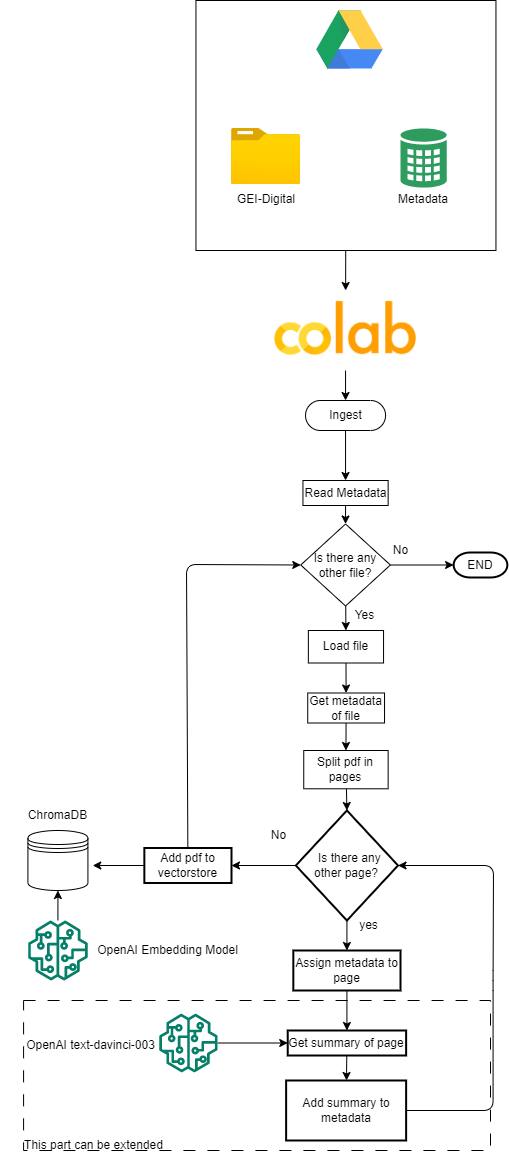
\includegraphics[height=0.5\pdfpageheight]{images/ingest.png}\label{fig:ingest}
    \caption[Ingestion]{Il diagramma di flusso che descrive la fase di ingest dei dati.}
\end{figure}

Come si può osservare, i dati sono stati conservati su Google Drive e il job di ingestion si occupa di leggere i 33 libri in formato pdf,
suddividerli in pagine assegnando loro le informazioni derivanti dai metadati, è presente inoltre una parte di enrichment di tali informazioni 
utilizzando il Large Language Model ``text-davinci-003'' di OpenAI per estrarre un riassunto di ogni pagina. Quest'ultima parte di enrichment è possibile espanderla ulteriormente
utilizzando l'LLM per estrarre ulteriori informazioni, come ad esempio le entità presenti in ogni pagina, ma per il momento è stata tralasciata.
La fase di enrichment inoltre serve ad arricchire i metadati di informazioni che, in seguito, il self-query retriever potrà utilizzare per interrogare il database.

Alimentato il database con le informazioni estratte, è possibile passare alla fase di inferenza.

\subsection[Inferenza]{Inferenza e interazione con l'utente}

La fase di inferenza e interazione con l'utente è descritta dal diagramma di flusso in figura 4.2:

\begin{figure}[H]
    \centering
    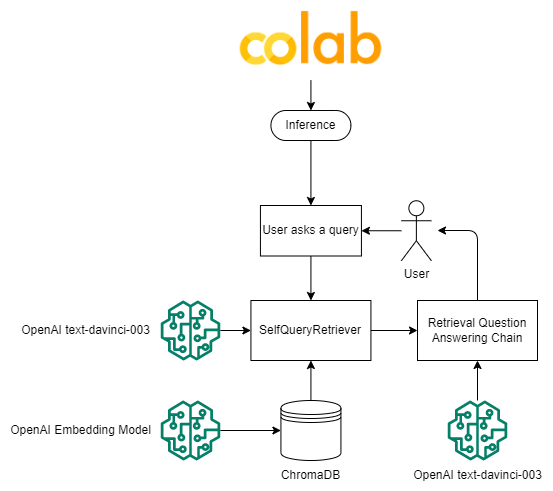
\includegraphics[height=0.3\pdfpageheight]{images/Inference.png}\label{fig:infer}
    \caption[Ingestion]{Il diagramma di flusso che descrive l'interazione dell'utente con il sistema di question answering.}
\end{figure}

Il job di inferenza si occupa di ricevere dall'utente una query in linguaggio naturale, la query passa in input al SelfQueryRetriever, 
che si occupa di interrogare il database e tramite una combinazione di selfquerying (riferimento ~\ref{fig:selfquery}) e similarity research restituisce una lista di documenti.
\begin{figure}
    \centering
    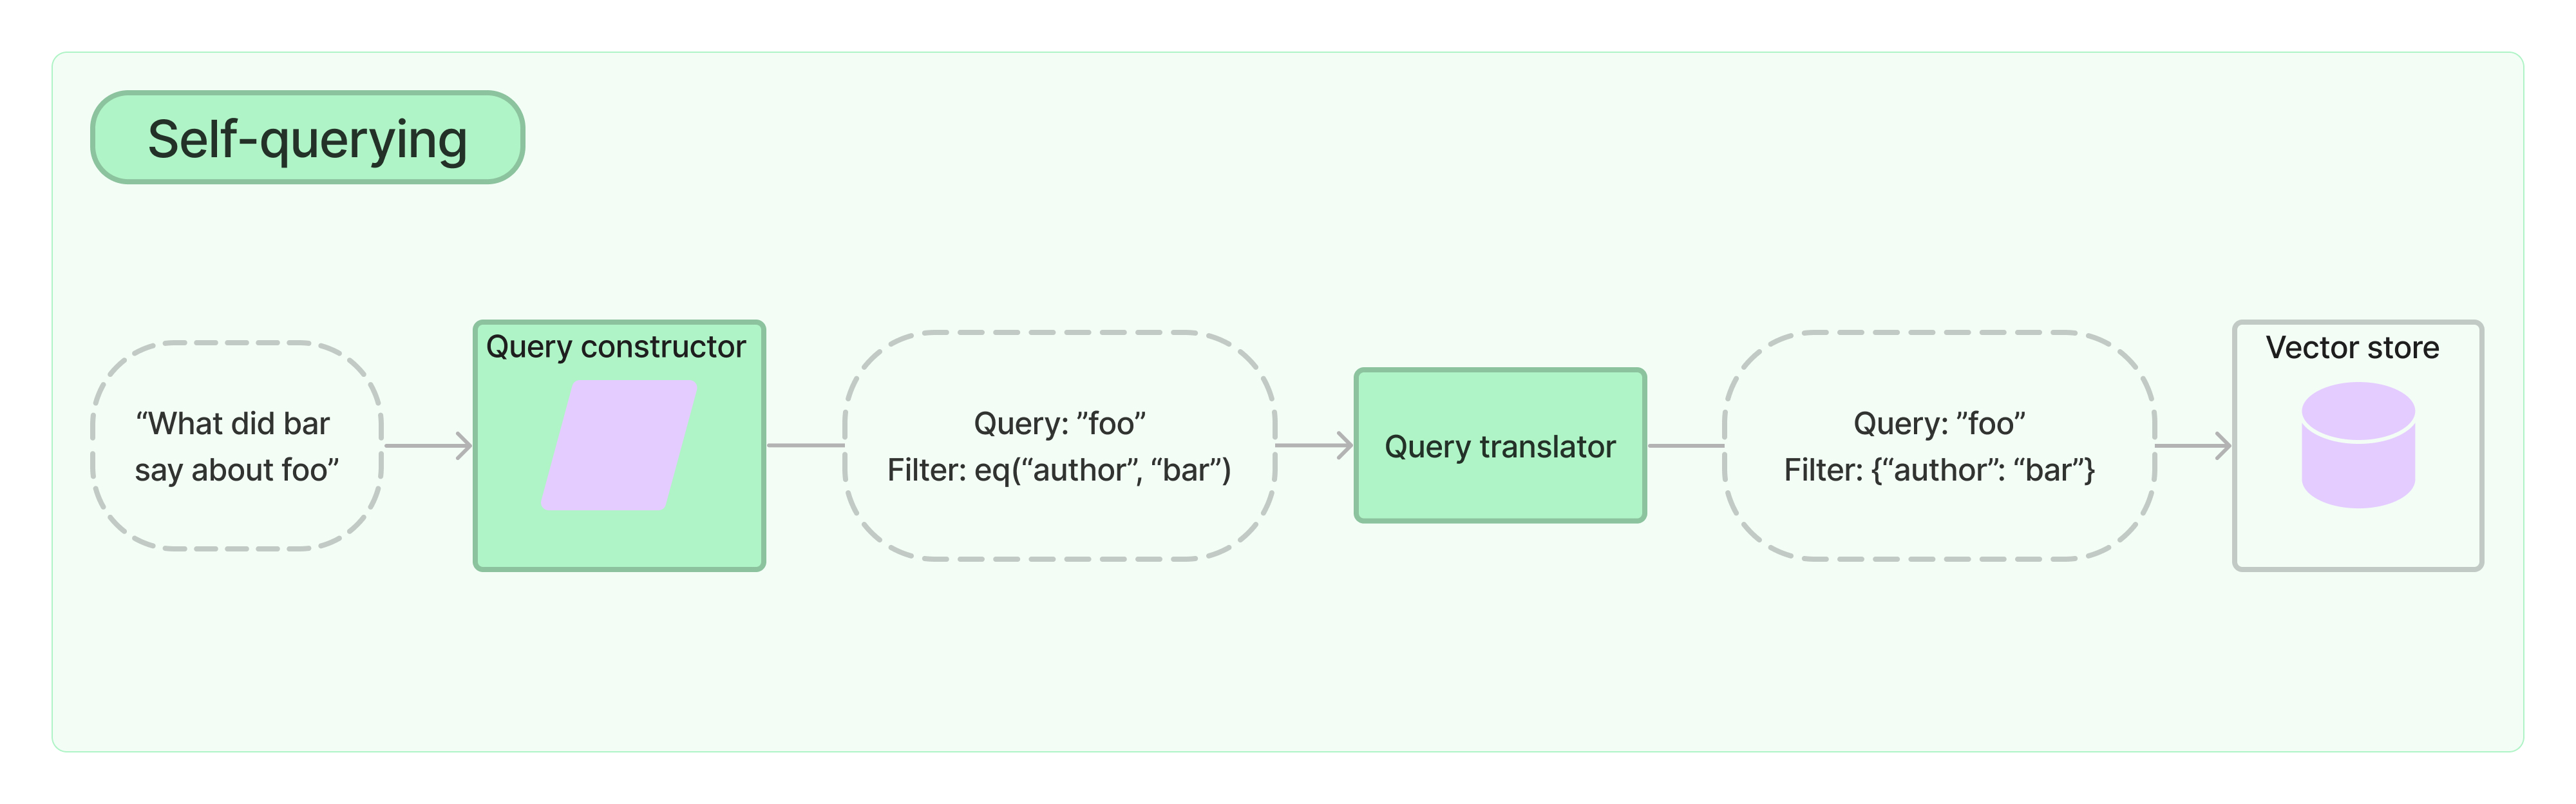
\includegraphics[width=0.7\pdfpagewidth]{images/selfquery.jpg}\label{fig:selfquery}
    \caption[Ingestion]{Come funziona un sistema di selfquerying.}
\end{figure}

Tali documenti vengono poi passati ad una catena di question answering, come contesto e, nella implementazione scelta, vengono presi in considerazione dal modello di OpenAI ``text-davinci-003'' che ciclicamente migliora la risposta precedente (figura \ref{fig:refine}).
In output vengono restituiti i documenti che il modello ha preso in considerazione e la risposta finale.

\begin{figure}
    \centering
    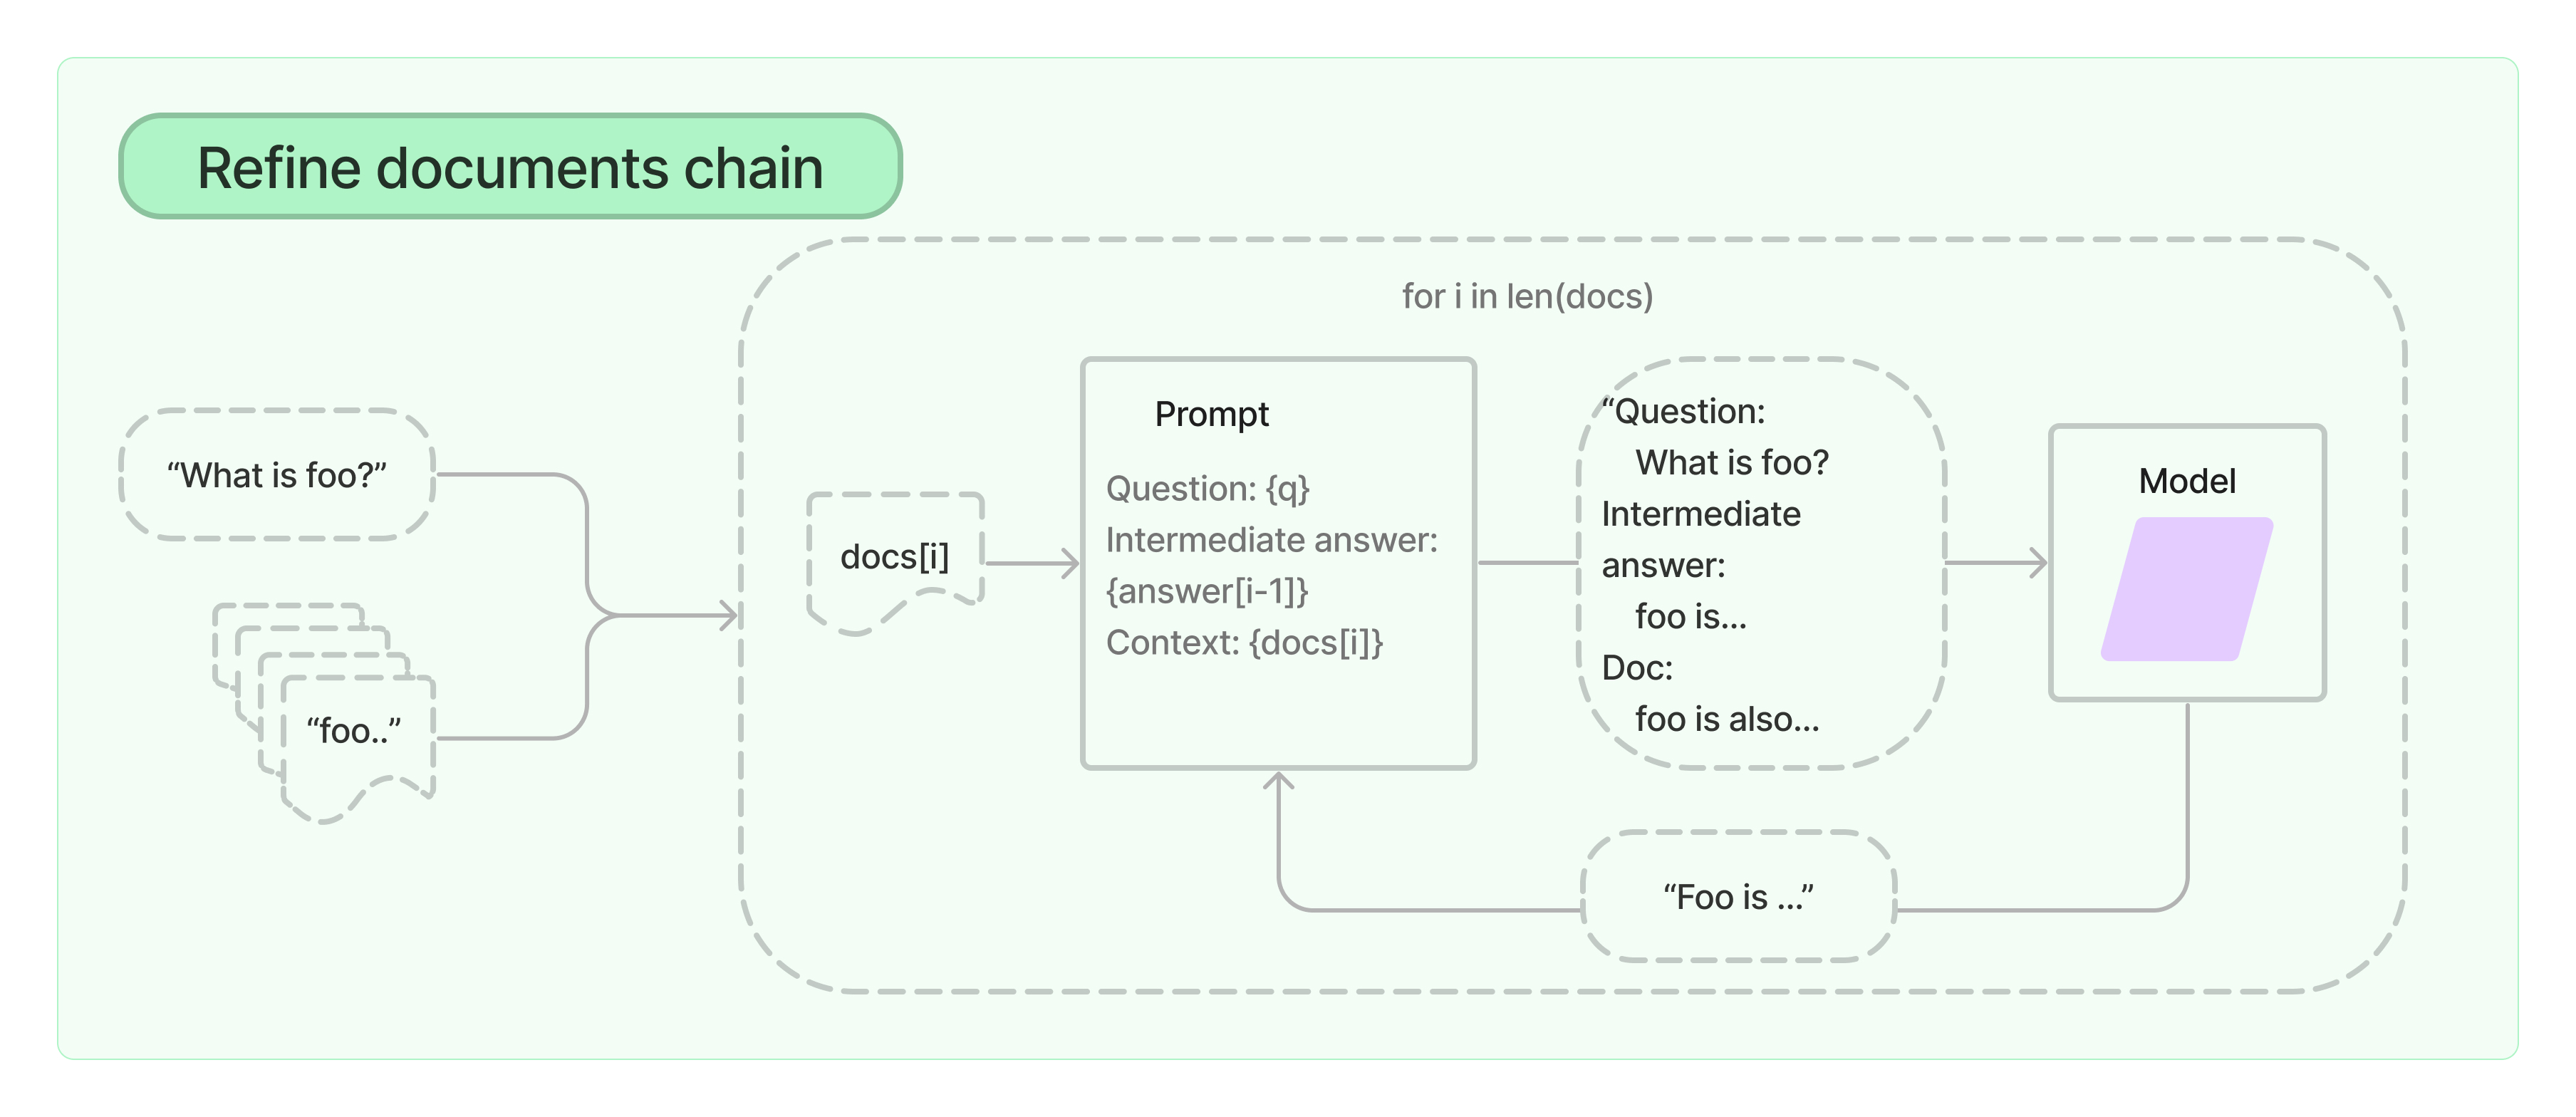
\includegraphics[width=0.7\pdfpagewidth]{images/refine.jpg}\label{fig:refine}
    \caption[Ingestion]{Come funziona una chain di tipo refine.}
\end{figure}


\section{I risultati}
\section{Costi}
I costi di un sistema di information retrieval basato su LLM possono essere divisi in due tipologie: fissi e di utilizzo.

I costi fissi sono quelli che non dipendono dal numero di query effettuate, ma solo dal numero di documenti indicizzati e dalla loro lunghezza.

Per il lavoro di tesi sono state utilizzate le API di OpenAI per semplicità di utilizzo e anche perché non richiedono capacità computazionali in loco.

Le api di OpenAI inoltre hanno un diverso costo rispetto al modello utilizzato. 

Il costo di indicizzazione utilizzando i modelli di OpenAI è di:

\begin{center}
    \begin{tabular}{|c|c|}
        \hline
        Model	& Usage \\
        \hline
        Ada v2	& \$0.0001\/1000 tokens \\
        \hline
    \end{tabular}
\end{center}

OpenAI stessa mette a disposizione altri modelli di embeddings ma ne sconsiglia l'utilizzo.

Il costo totale dell'indicizzazione è stato intorno ai 60\$.

Per quanto riguarda invece il costo di utilizzo, OpenAI mette a disposizione diversi modelli con diversi costi descritti nella tabella seguente:

\begin{center}
    \begin{tabular}{|c|c|c|c|}
        \hline
        Family & Model	& Input cost & Output cost \\
        \hline
        GPT-4 & 8k context	& \$0.03 / 1000 tokens &  	\$0.06 / 1000 tokens \\
        \hline
        & 32k context	& \$0.06 / 1000 tokens &  	\$0.12 / 1000 tokens \\
        \hline
        GPT-3.5 Turbo & 4k context	& \$0.0015 / 1000 tokens &  	\$0.002 / 1000 tokens \\
        \hline
        & 16k context	& \$0.003 / 1000 tokens &  	\$0.004 / 1000 tokens \\
        \hline

        GPT-3 & davinci	& \$0.0120 \/ 1000 tokens &  	\$0.0120  \/ 1000 tokens \\
        \hline
    \end{tabular}
\end{center}



Se si fosse utilizzato un modello di LLM proprietario o di terze parti in modo diretto sarebbe stato necessario un server con una GPU per poter effettuare le query in modo efficiente. In tal caso i costi si sarebbero ammortizzati sul lungo periodo.



\section{Le conclusioni}
	\printbibliography[heading=bibintoc]
\end{document}